\documentclass[a4paper]{article}

\usepackage{times}
\usepackage{t1enc}
\usepackage[french]{babel}
\usepackage{graphicx}

\title{L'algorithme de plus court chemin sous contraintes d'EuG\`ene}
\author{T. Schiex}

\begin{document}
\maketitle

Je me place dans le cas du graphe $G=(S,A)$ d'EuG\`ene qui est form\'e
d'une s\'erie de pistes parall\`eles. Je noterai $s_{ik}$ le $i$\`em sommet
de la piste $k$. Les poids des ar\^etes entre les sommets de la position
$i$ et de la position $i+1$ et des pistes $k$ et $k'$ respectivement
est not\'e $w_{ikk'}$ (\'egal \`a $+\infty$si il n'y a pas d'ar\^ete dans le
graphe). La nature des arcs entre les positions $i,i+1$ et $i+1,i+2$
est diff\'erente (ar\^ete de contenu et de signaux respectivement) mais
nous n\'egligerons ce d\'etail. 

\begin{figure}
\begin{center}
  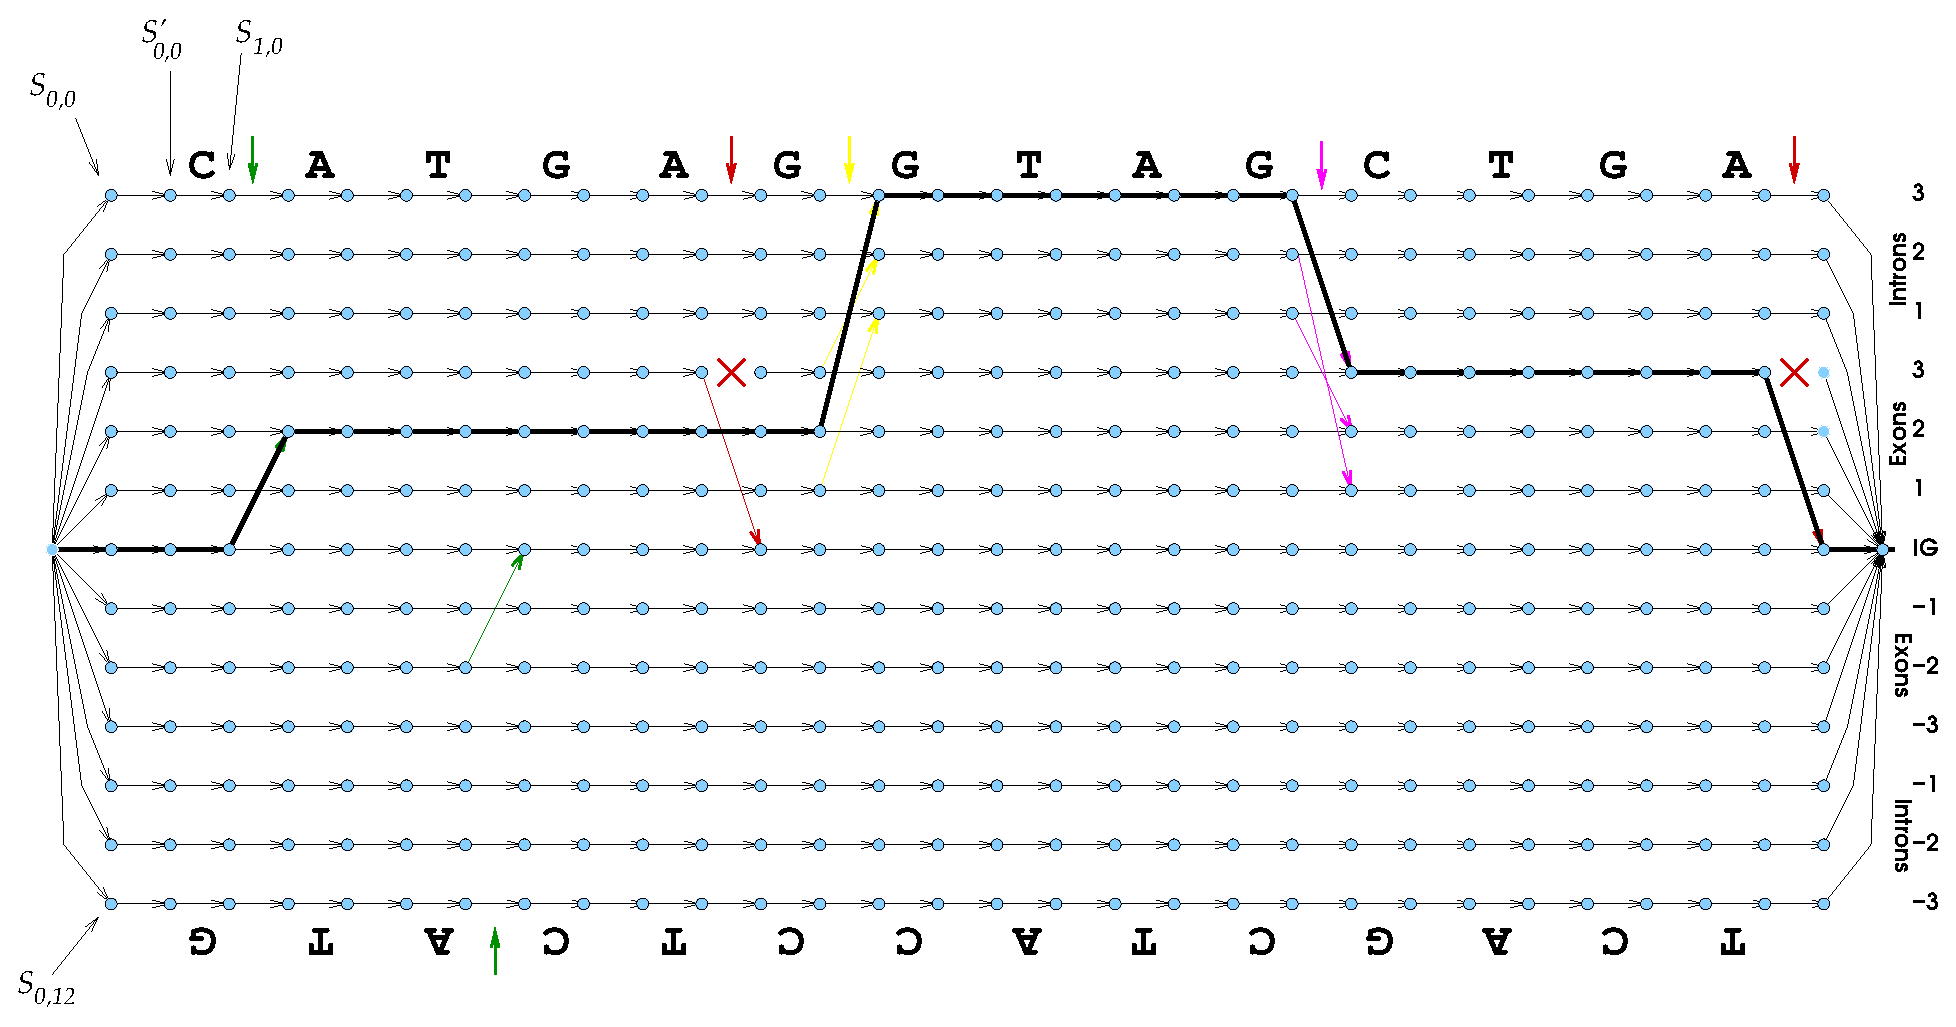
\includegraphics[width=\textwidth]{graph}
\end{center}
\end{figure}

Si l'on se contente de calculer le plus court chemin qui va de la
source au puits, il est obtenu simplement par une r\'ecurrence. On note
$SP[s]$ pour tout sommet $s$ la longueur du plus court chemin de la
source \`a $s$ et $\pi[u]$ le sommet qui doit \^etre utilis\'e pour
atteindre $s$ par un plus court chemin.

Supposons que l'on connait $SP[]$, le co\^ut du plus court de la source
aux $i$\`eme sommets (initialement vrai pour $i=0$). On peut calculer la
valeur de $SP[]$ pour les sommets \`a la position $i+1$ par une simple
r\'ecurrence:

\[SP[s_{i+1,k}] = \min_l \{ SP[s_{i,l}+w_{ikl}\}\]
\[\pi[s_{i+1,k}] = arg\min_l \{ SP[s_{i,l}+w_{ikl}\}\]

qui consiste \`a dire que le plus court chemin pour aller au sommet
$s_{i+1,k}$ est obtenu en allant \`a un sommet qui pr\'ec\`ede par un plus
court chemin puis en rejoignant le sommet $s_{i+1,k}$ et ce en
choisissant le sommet pr\'ec\'edant qui m\`ene \`a un co\^ut minimum (principe
d'optimalit\'e de Belmann).

On souhaite prendre en compte des contraintes de longueur minimum,
d\'efinie par une longueur minimum $\ell$ et un num\'ero de piste $k$. Pour
tout chemin source-puits dans le graphe de pr\'ediction, on dira qu'il
viole $\langle\ell,k\rangle$ s'il contient un sous-chemin $\langle
u_0,u_1,\ldots,u_{m-1},u_m\rangle$ tel que~:
\begin{itemize}
\item $u_0$ n'est pas la source et ne se situe pas sur la piste $k$,
\item $u_m$ n'est pas le puits et ne se situe pas sur la piste $k$,
\item pour tous les sommets $u_i, 1\leq i\leq m-1$, la piste de $u_i$
  est $k$,
\item enfin, $m-1 < 2\ell$
\end{itemize}

Un tel sous-chemin est dit en violation, l'ar\^ete $(u_0,u_1)$ est son
ar\^etre ouvrante et $(u_{m-1},u_m)$ son ar\^ete fermante. Une chemin est
faisable s'il ne contient aucun sous-chemin en violation avec une
contrainte.

\'Etant donn\'e un graphe de pr\'ediction et un ensemble de contraintes de
longueur, trouver un plus court chemin faisable de la source au puits
peut encore se faire par r\'ecurrence. Il suffit de remarquer sur si
l'on connait $SP[]$, la longueur d'un plus court chemin faisable pour
les $i$\`eme sommets et ce pour $i$ allant de $0$ \`a $j$, il est possible
de d\'eterminer la longueur d'un plus court chemin faisable pour les
$j+1$\`eme sommets par r\'ecurrence.

Consid\'erons une ar\^ete qui relie le sommet $s_{j+1,k}$ \`a un sommet
pr\'ec\'edant $s_{j,k'}$~:
\begin{itemize}
\item Si $k=k'$ alors le prolongement du chemin faisable le plus court
  de la source \`a $s_{j,k'}$ par cet ar\^ete d\'efinit aussi un chemin
  faisable, qui est le plus court parmi tous ceux passant par
  $s_{j,k'}$ (Belmann).
\item Sinon, cette ar\^ete peut \^etre l'ar\^ete fermante d'un sous-chemin
  violant une contrainte li\'ee \`a la piste $k'$ que l'on quitte. Les
  seuls chemins faisables passant par $s_{j,k'}$ doivent alors rester
  au moins pour $\ell$ sommets sur la piste $k'$ ou venir directement de
  la source par la piste $k'$. Soit $s= s_{j-\ell,k'}$ le sommet situ\'e
  sur la piste $k'$ en position $j-\ell$ (s'il existe, $s$ sera pris
  \'egal \`a $s_{0,k'}$sinon). Alors tous les chemins faisables qui
  arrivent en $s_{j+1,k}$ par $s_{j,k'}$ passent par $s$. En utilisant
  le principe de Belmann, on prouve que les chemins faisables les plus
  courts qui arrivent en $s_{j+1,k}$ par $s_{j,k'}$ sont obtenus en
  prolongeant le plus court chemin faisable de la source \`a $s$ par un
  chemin de $s$ \`a $s_{j,k'}$ restant sur la piste $k'$.
\end{itemize}

Si l'on note $L(j,\ell,k')$ la longueur du chemin qui part de ce sommet
$s= s_{\max(0,j-\ell)k'}$ et qui aboutit \`a $s_{j,k'}$ en restant sur la
piste $k'$, la r\'ecurrence pour calculer $SP[]$ est simplement:

\[SP[s_{j+1,k}] = \min(SP[s_{j,k}]+w_{jkk} , \min_{k'\neq k} \{ SP[s_{\max(0,j-\ell)k'}]+L(j,\ell,k')+w_{jk'k}\} \]

Lorsque le plus court chemin est obtenu par le premier terme
$SP[s_{j,k}]+w_{jkk}$, il est simple de m\'emoriser le plus court chemin
qui m\`ene \`a $s_{j+1,k}$ ~: il est obtenu en passant par $s_{j,k}$.
Sinon, il est plus complexe car il est obtenu en passant par
$s_{j,k'}$ et en restant sur la piste $k'$ jusqu'\`a
$s_{\max(0,j-\ell)k'}$ puis en utilisant le chemin indiqu\'e par
$\pi[s_{\max(0,j-\ell)k'}]$. C'est pour cette raison que la classe
\texttt{BackP} a \'et\'e con\c cue.

\section{La classe \texttt{BackP}}

La classe forme une liste doublement cha\^\i n\'ee (champs \texttt{Next} et
\texttt{Prev}). Chaque \texttt{BackP} est charg\'e de repr\'esenter une
succession d'ar\^etes (un sous-chemin) du graphe d'EuG\`ene. 

Le champ \texttt{State} m\'emorise le num\'ero de piste qui correspond au
sous-chemin. Le champ \texttt{SwitchType} m\'emorise le type
d'aiguillage (un Start, un Stop, un site d'\'epissage\ldots) qui marque le
d\'ebut du sous-chemin, le champ \texttt{StartPos} marque la position
(en terme de nucl\'eotides) du d\'ebut du sous-chemin, La somme de
\texttt{Cost} et \texttt{d'Additional} donne le co\^ut du meilleur
chemin de la source jusqu'\`a la derni\`ere position repr\'esent\'ee par le
sous-chemin (\texttt{Cost} seul repr\'esente le co\^ut d'un plus court
chemin jusqu'\`a la premi\`ere position du sous-chemin). Enfin, le
sous-chemin repr\'esent\'e par une instance de \texttt{BackP} se prolonge
par le sous-chemin repr\'esent\'e par le \texttt{BackP} point\'e par
\texttt{Origin}.

Initialement, on instancie un BackP par piste (18 instances) stock\'ees
dans le tableau \texttt{LBP} (Liste de BackP). Ces premi\`eres instances
serviront de marqueurs de fin de liste est sont donc sp\'ecifiques~:
\begin{itemize}
\item \texttt{StartPos} vaut -1,
\item \texttt{Prev} et \texttt{Next} pointent tous deux sur l'instance
  elle-m\^eme.
\end{itemize}

Pour conna\^\i tre le meilleur chemin qui m\^ene a un sommet donn\'e \`a partir
d'une piste donn\'ee, il suffit d'utiliser les fonctions
\texttt{BestUsable} et \texttt{StrictBestUsable}. Sans rentrer dans
les d\'etails, ces fonctions vont parcourir la liste des \texttt{BackP}
(donc la s\'equence en arri\`ere) correspondant \`a une piste pour trouver
le premier BackP qui commence assez loin de la position courante (pour
respecter la contraite de longueur impos\'ee par \texttt{len}) et
retourner le co\^ut correspondant dans \texttt{cost} ainsi que le
\texttt{BackP} correspondant.

S'il s'av\`ere que le meilleur chemin (selui de co\^ut le meilleur) pour
arriver \`a un sommet consiste \`a faire autre chose que de continuer sur
la m\^eme piste, on va cr\'eer une nouvelle instance de \texttt{BackP}
avec \texttt{InsertNew} en indiquant la position courante comme
position de d\'emarrage, l'\'etat dont l'on vient comme ``\'etat'', le type
d'aiguillage utilis\'e, le co\^ut et le BackP qui indique le sous-chemin
optimal identifi\'e.

Sinon, si le meilleur chemin consiste juste \`a rester sur la m\^eme
piste, on ``allonge'' simplement l'instance \texttt{BackP} courante
via la fonction \texttt{Update} qui incr\'emente \texttt{Additional}.

Quand on a fini d'analyser la sequence il suffit de consulter les
co\^uts des 18 LBP[], de choisir celui de co\^ut le meilleur et
d'encha\^\i ner les sous-chemins repr\'esent\'es par les \texttt{BackP} en
s\'equence, en suivant les \texttt{Origin}.

\section{Ajouter les Frameshifts}

Un frameshift permet de changer de phase, avec insertion ou d\'el\'etion
d'un nucl\'eotide. Il s'agit donc juste d'un nouvel aiguillage entre
pistes codantes d'un m\^eme brin. La seule difficult\'e provient d'une
interaction entre les contraintes minimum de longueurs et les
frameshifts.

Lorsque le meilleur chemin qui aboutit \`a un sommet d'une piste exon
utilise un frameshift, les contraints de longueur minimum des exons
vont garantir que la partie de l'exon avant et apr\`es le frameshift
vont avoir toutes les deux une longueur sup\'erieure au minimum
autoris\'e. Globalement un exon avec des frameshifts aura donc un
longueur minimum \'egal \`a la longueur minimum normale multipli\'ee par le
nombre de frameshifts plus un.

Pour l'instant, comme les frameshifts sont rares et que la longueur
minimum d'un exon est faible, on consid\`ere que ca ne pose pas de
probl\`eme. Le mieux serait de pouvoir raisonner sur des longueurs
minimum pour des classes de pistes (tous les exons forward).

\end{document}
